
%(BEGIN_QUESTION)
% Copyright 2007, Tony R. Kuphaldt, released under the Creative Commons Attribution License (v 1.0)
% This means you may do almost anything with this work of mine, so long as you give me proper credit

In Fieldbus function block programming, signals are linked from one function to another by lines drawn between the respective inputs and outputs.  An example of this is the following {\it cascade} PID control strategy, where the output of one PID controller (the ``master'') determines the setpoint for another PID controller (the ``slave'').  Lines drawn between the function blocks show which outputs connect to which inputs:

$$\includegraphics[width=15.5cm]{i02443x01.eps}$$

An important concept to grasp in Fieldbus function block programming is that these connections not only carry signal values, but signal {\it statuses} as well.  That is, each signal in a function block programming environment carries with it a status code to indicate how valid that signal is.

\vskip 10pt

Identify the three status conditions for signals in a FOUNDATION Fieldbus system, and also explain what the term {\it status propagation} means with reference to function block programming.

\vskip 20pt \vbox{\hrule \hbox{\strut \vrule{} {\bf Suggestions for Socratic discussion} \vrule} \hrule}

\begin{itemize}
\item{} A useful analytical technique for any complex control system is to annotate the diagram with arrowheads showing the directions of all data pathways between devices or functions.  Show how this helps you analyze the control strategy diagram shown in this question.
\item{} For those who have studied {\it cascade control} strategies, identify which of the PID function blocks is the master and which is the slave in this FF function block program.
\item{} What status value does the output of a block placed into ``manual'' mode carry?
\item{} What status value does the output of a block placed into ``out of service'' mode carry?
\item{} Suppose the valve positioner executing the AO function block experiences a problem, causing its BKCAL\_OUT signal to switch to a ``Bad'' status value.  How will this status change affect the operation of this function block program?
\item{} Suppose the slave PID function block is switched into Manual mode.  How will this mode change affect the operation of this function block program?
\end{itemize}

\underbar{file i02443}
%(END_QUESTION)





%(BEGIN_ANSWER)

The three status conditions are easy to research -- I'll let you do that!  Status propagation means that the status of a signal will ``propagate'' from the originating function block to subsequent function blocks in the program so that they make take appropriate actions.

%(END_ANSWER)





%(BEGIN_NOTES)

The three valid status conditions of Fieldbus signals are:

\begin{itemize}
\item{} Good
\item{} Bad
\item{} Uncertain
\end{itemize}

Signals also carry {\it sub-status} information providing more detail on the nature of the status.

\vskip 10pt

For an example of status propagation, a ``Bad'' status from the master analog input will automatically switch the master PID controller to {\it manual} mode.  This is a default response of the PID function block (see page 9-9 of Emerson's {\it Foundation Fieldbus Blocks} document, number 00809-0100-4783).

\vskip 10pt

Fieldbus function blocks placed into manual mode generally propagate ``Good'' status values, to enable a manually-fixed value to be used for diagnostic purposes without causing downstream function blocks to shed into abnormal modes.  It may be possible, however, for the user to configure a function block such that its output status sheds to {\it Uncertain} when placed into manual mode (see the {\tt STATUS\_OPTS} parameter of the AI function block for a discussion of this option).  If a function block is placed into the ``out of service'' mode, the status will switch to {\it Bad : Out Of Service}.




\vfil \eject

\noindent
{\bf Prep Quiz:}

Identify the three status conditions of FOUNDATION Fieldbus signals:

\begin{itemize}
\item{} Nominal, Faulty, and Intermediate
\vskip 5pt 
\item{} Good, Bad, and Uncertain
\vskip 5pt 
\item{} Functional, Faulty, and Unreliable
\vskip 5pt 
\item{} Excellent, Poor, and Unstable
\vskip 5pt 
\item{} Nominal, Poor, and Changing
\vskip 5pt 
\item{} Good, Bad, and Ugly
\end{itemize}


%INDEX% Fieldbus, function block: signal status
%INDEX% Fieldbus, function block: status propagation

%(END_NOTES)


